%!TEX root = ../template.tex
%%%%%%%%%%%%%%%%%%%%%%%%%%%%%%%%%%%%%%%%%%%%%%%%%%%%%%%%%%%%%%%%%%%
%% chapter1.tex
%% NOVA thesis document file
%%
%% Chapter with introduciton
%%%%%%%%%%%%%%%%%%%%%%%%%%%%%%%%%%%%%%%%%%%%%%%%%%%%%%%%%%%%%%%%%%%


\chapter{Methodologies}
\label{cha:methodologies}
Taking into account the existing usability problems and the target users' requirements and expectations, a methodology was essential in order to design, implement, and evaluate solutions throughout the development process. Therefore, this chapter will present the multiple phases and techniques carried out since the first sketches to the final evaluations.

\section{Iterative Design}
\label{sec:iterative_design}
Before starting the solution building process, the phases were planned for the sake of the development of the final solution. Accordingly, it will be presented the design strategy adopted, which will be further detailed in \nameref{cha:design_and_implementation}. The chosen methodology uses an iterative design strategy in order to keep a user-centric design, which prioritizes the users' needs according to the mentioned in \ref{subsec:user_centered_design}. Regarding the prototyping method, the evolutionary prototyping principle (described in \ref{subsubsec:sketching_and_prototyping}) was applied, where the last prototype was used as a baseline to develop the prototype of the next iteration.

\textbf{Sketching: }The design process started with an initial sketching phase, where the first solution ideas were explored and drafted. In this technique, the integration of new ideas into the existing interface is favored given the fact it is an interactive process where the ideas are tested progressively. The most important aspect was to think about system transversal changes and not about particular details of specific components, since these details could be refined later. The outcome of this phase sets a more concrete idea of what can be inserted in the prototype, even if it is necessary to think more about how to implement it later.

Keeping in mind the ideas explored in the sketching phase, it is possible to start to build the prototypes that will be tested by users. The first decision taken was how many prototypes should be built taking into consideration the resources and time available. As mentioned in \ref{subsubsec:sketching_and_prototyping}, the first prototypes should be low-fidelity prototypes, and iteration by iteration, this level should increase in order to refine details in the interface. In that way, it was decided to build two prototypes:

\begin{itemize}
    \item \textbf{Paper Prototype: } Simple low-fidelity prototype implemented in paper using a ruler, a set square, and writing materials. Through that approach, it is possible to implement the first ideas faster and reduce the risk of adoption failure, since the implemented ideas were already tested. The main concern of this type of prototype is that the design of the major interface changes might affect users mental model which enables the early detection of which choices should continue to the next iterations or if they need to be redesigned.
    \item \textbf{Service Studio Prototype: } This is the final prototype, developed using C\#, Typescript \cite{typescript}, and React \cite{react}, which is integrated in the new Design of the Service Studio. Through this prototype, the solutions implemented were validated and compared with the previous existing implementation in order to validate if the usability of the system has improved with the implemented changes.
\end{itemize}

In each one of the two above-mentioned prototypes, it was included the following phases: design, implementation, and evaluation. In the Design phase solution ideas that could be applied were set up as well as the priorities to be tackled in the prototype. The Implementation phase refers to the concrete prototype development process. Finally, in the Evaluation phase, the prototypes were tested by end-users, according to the testing approach further explained in \ref{sec:testing_scenarios} and \ref{sec:evaluation_method}.

Regarding evaluation, it was necessary to establish how many users should be tested in each evaluating phase. In these phases, not only the two mentioned prototypes were considered, but also the evaluation of the existing interface mentioned in \ref{sec:current_implementation_evaluation}. 

The data of that analysis is also an opportunity to has a baseline of the development starting point across the solution building. Thereby, the number of users tested in the first prototype is also an important factor.

Nielsen performed some studies quantifing how many users should be tested in a usability study, leading to the conclusion that 5 users were a sufficient number for a qualitative studies since it is possible to get the maximum benefit-cost ratio - "Testing with 5 people lets you find almost as many usability problems as you'd find using many more test participants" \cite{why_you_only_need_to_test_with_5_users} \cite{how_many_test_users_in_a_usability_study}. However, to perform quantitative analysis it is necessary to get at least 20 users in order to get statistical relevance \cite{how_many_test_users_in_a_usability_study}.

According to the studies mentioned, at least 5 users of each user group (described in \ref{sec:target_users}.) should be tested since only a qualitative analysis will be performed to validate user's interaction with the applied changes. Nevertheless, some statistical results should be also subject of analysis in order to compare if the new solution provide improved usability than the existing version. Hence, it was decided to test more users in the existing implementation and in the final prototype in order to obtain enough elements to conduct a quantitative analysis. In that way, Table \ref{tab:number_of_users_tested_by_each_user_group_and_solution} shows how many users were tested by each user group and by each solution evaluated.

\begin{table}[tb]
	\caption{Number of users tested by each user group and by each solution evaluated}
	\label{tab:number_of_users_tested_by_each_user_group_and_solution}
\centering
\resizebox{\textwidth}{!}{
\begin{tabular}{c|c|c|c|c|}
    \cline{2-5}
    \rowcolor[HTML]{C0C0C0} 
    \cellcolor[HTML]{FFFFFF}                                 & Previous Implementation & Paper Prototype & Service Studio Prototype & Total \\ \hline
    \multicolumn{1}{|c|}{\cellcolor[HTML]{C0C0C0}OutSystems Developer}    & 10         & 5               & 10                    & 25 \\ \hline
    \multicolumn{1}{|c|}{\cellcolor[HTML]{C0C0C0}Software Developer} & 10        & 5              & 10                   & 25\ \\ \hline
    \multicolumn{1}{|c|}{\cellcolor[HTML]{C0C0C0}Citizen Developer} & 10        & 5              & 10                   & 25\ \\ \hline
    \multicolumn{1}{|c|}{\cellcolor[HTML]{C0C0C0}Total} & \textbf{30}        & \textbf{15}              & \textbf{30}                   & \textbf{75}\ \\ \hline
    \end{tabular}
    }
\end{table}

To compare the different phases, all tests were performed using the same testing scenarios, which are presented in the following section.


\section{Testing Scenarios}
\label{sec:testing_scenarios}
Given the wide scope of the usability problems identified, a plan of the testing approach was required in order to evaluate the most important aspects of the user-interface communication, given the short period available to test the users. Following the plan, it was possible to keep the testing focus on the prioritized details in a feasible way.

Firstly, it was defined the type of testing scenarios that would be presented. For that decision, it was taken into account the specific aspects that should be improved in the interface usability. As mentioned, not only the optimization of the efficiency, effectiveness, learnability, and user satisfaction of the entire query formulation process was the goal, but also the improvement of the query comprehension. In such a way that it was important to evaluate if users could understand the query purpose (i.e., what data intends to be fetched from the database) as well as the time they required to realize that.

Considering those evaluation requirements, two types of testing scenarios were prepared: scenarios where users explore an existing query and try to realize what was its purpose, and the other ones where users try to formulate it on their own. Through that approach, it was possible to analyze the usability of the interfaces tested for both points of view: comprehension and formulation.

Nevertheless, the complexity of the queries presents a crucial factor when the scenarios were thought out. For example, an interface could be useful and pleasant to use in simple use cases but it could lead to a decrease of that quality in more complex queries. Accordingly, is was listed the requirements that were considered relevant to be covered by user testing scenarios:

\begin{itemize}
    \item \textbf{Query Comprehension: }Relevant aspects that should be present in the queries and consequently in the interface to evaluate, as extensive as possible, queries' comprehension:
    \begin{itemize}
        \item \textbf{Interface Elements Exploration: }Include use cases that contain the majority of the query components supported by the system: database entities and joins of different types, filtering and sorting criteria applied to different data types, and other query components added throughout the query formulation process, such as Group Bys, Aggregation Functions (SUM, MIN, MAX, AVG, COUNT) or Calculated Attributes \footnote{These operations were presented in \ref{subsubsec:current_progress}};
        \item \textbf{Joins Representation: }Representation of different joins in order to analyze if users could successfully identify them. First of all, there was a concern to consider in the scenarios joins of different types, such as inner joins or left joins. It was important to consider not only the most common joins (i.e., joins where the unique foreign key referencing another table is equals to the other table primary key) but also some queries that contain joins with more advanced conditions. For instance, when the join between two tables could be made using different foreign keys, as they are multiple relationships between both tables, or when the join condition contains logical operators.
    \end{itemize}
    \item \textbf{Query Formulation: }At the same time, the following aspects were considered essential to be approached in the user testing scenarios from a query formulation point of view:
    \begin{itemize}
        \item \textbf{Add Data Sources and Joins: }Identify the options chosen to add query sources and analyze what are the users' reactions to the system automatisms to simplify the joins specification;
        \item \textbf{Edit Query Filters: }Evaluate if the query filters edition is intuitive and what barriers could exist in the interfaces regarding this aspect;
        \item \textbf{Insert Calculated Attributes, Group Bys, and Aggregation Functions: }Check if users could understand the cases where they would need to use the referred functionalities and if they can discover how to apply them without difficulty;
        \item \textbf{Use Hidden Columns: }Verify the main difficulties identified by users when they need to apply actions in attributes that were not entirely visible in the interface, either because they are hidden, or because they are not visible due to the lack of available space in the interface (scroll required).
    \end{itemize}
\end{itemize}

The aspects mentioned were considered the most relevant to analyze since they allow a widespread use of the tool but they also cover multiple cases identified as critical in terms of usability, according to the aspects detailed in \ref{sec:problem_definition}.

Nevertheless, the data model could have also a significant impact on user testing results. For instance, if a user does not understand the data model, he could miss the purpose of the query, even if the query is presented in a simple and readable manner. In that way, the selection of the data model used for user testing was performed attending to the following points:

\begin{itemize}
    \item \textbf{Simple Business Domain: }The data stored in the database should represent an example of a day-to-day application that could be understandable by any user regardless of his background.
    \item \textbf{Different data types: }The data model should contain a wide variety of data types since it could become useful in order to reflect if the design approaches chosen are able to work with different types of data;
    \item \textbf{Multiple relationships between two entities: }The interface aims to accelerate and simplify the querying process not only for simple cases. For this reason, it is important to perceive how the interface could help users in cases where there are more than one relationship between two entities. Moreover, \gls{SQL} does not have any particular syntax that helps users in these cases, then there is an improvement opportunity here.
\end{itemize}

\begin{figure}[htbp]
	\centering
	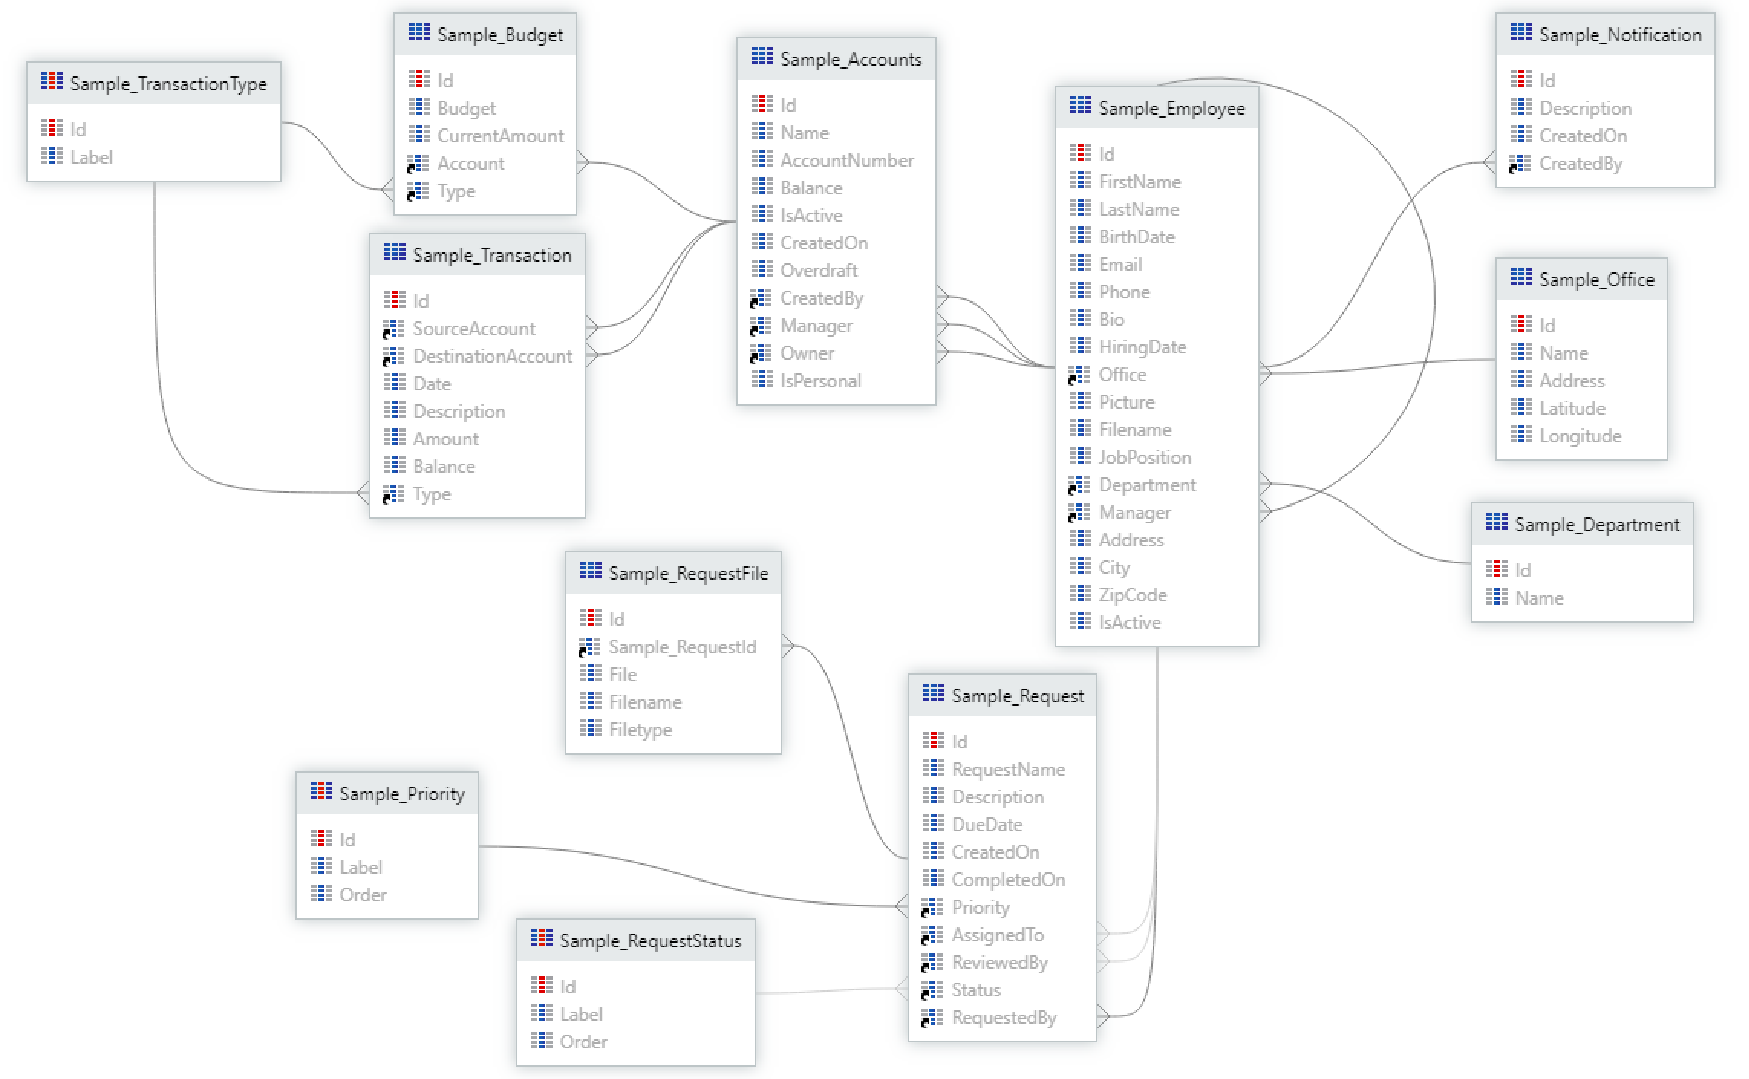
\includegraphics[height=3.6in]{data-model}
	\caption{Data Model used for User Testing}
	\label{fig:dataModel}
\end{figure}

Accordingly, \ref{fig:dataModel} illustrates the data model of the database adopted to perform all usability tests.

After choosing the data model used as support for the usability tests, the list of test scenarios was elaborated. Three different types of scenarios were designed:

\begin{itemize}
    \item \textbf{Query Comprehension: } The user explores a visual query already built and tries to indicate what are the query components presented as well as the data that would be fetched from the database through that query;
    \item \textbf{Query Modification: } After a query comprehension example, the user tries to apply some modification on the existing query previously explored;
    \item \textbf{Query Formulation: } Given a natural language statement that explains what data is intended to be fetched from the database, the user tries to formulate a new visual query from scratch in order to retrieve the data intended.
\end{itemize}

Through that approach, it was possible to keep the focus on different aspects according to the scenario used. On the one hand, the comprehension scenarios give the focus to the query readability, which promote a global exploration of the query components and gave the opportunity to understand if users clearly identified the purpose of each interface section. On the other hand, modification and formulation scenarios were used to understand if users could built queries through the interface presented.

Nevertheless, there was several results to be obtained from the user testing scenarios and it was difficult reach an approach to test all aspects related to the existing problems in a short period. Since the testing requirements presented above must be integrated in the scenarios, a strategy was used to distribute the different requirements among the different scenarios in order to evaluate them all in a fluid and natural way for the user. 

%Considering the short period available to test all mentioned requirements, the aspects considered essential to be present in the use cases explored were combined in a table in order to distribute them along a set of scenarios. Figure X 

Therefore, Table \ref{tab:scenarios_complexity} was used to assign organize the complexity of each scenario and check the aspects that would be tested in each one.

\textbf{Table \ref{tab:scenarios_complexity} clarifications regarding the factors integrated in testing scenarios: }
\begin{itemize}
    \item \textbf{Simple Joins: }Joins that are automatically generated by the system without requiring human intervention;
    \item \textbf{Complex Joins: }Joins that need to be partially configured manually (e.g., to specify the foreign key used to merge both tables or to change the join condition);
    \item \textbf{Left Join with Null: }Left join between entities A and B, to consider only the entities A that are not related to B (e.g., the employees who have not created any notification.);
    \item \textbf{Group by (without reference): } The system has an automatism that generates automatically a name to a new attribute grouped by. However, this name is not self-explanatory and there was no reference to the source of its attribute. That way, it is important to highlight this case;
    \item \textbf{Aggregation Functions: } The aggregation functions supported by aggregates are Max, Min, Average, Sum, and Count. As the representation in the interface as well as the insertion method is similar, only a few of these were used;
\end{itemize}

\begin{table}[tb]
    \caption{Distribution of the relevant testing aspects among the testing scenarios designed.}
	\label{tab:scenarios_complexity}
    \begin{tabular}{|l|l|c|c|c|c|c|c|c|}
        \hline
        \multicolumn{2}{|l|}{\textbf{Scenarios}}                                                                                                                                                          & \multicolumn{1}{l|}{\textbf{C1}}           & \multicolumn{1}{l|}{\textbf{M1}} & \multicolumn{1}{l|}{\textbf{C2}}           & \multicolumn{1}{l|}{\textbf{C3}}           & \multicolumn{1}{l|}{\textbf{F1}} & \multicolumn{1}{l|}{\textbf{C4}}           & \multicolumn{1}{l|}{\textbf{M4}} \\ \hline
                                                                                                                               & Number of Entities                                                       & 4                                          & 4                                & 6                                          & 3                                          & 3                                & 5                                          & 7                                \\ \cline{2-9} 
                                                                                                                               & Simple Joins                                                             & 2                                          & 2                                & 4                                          & 2                                          & 1                                & 3                                          & 3                                \\ \cline{2-9} 
                                                                                                                               & Complex Joins                                                            & -                                          & -                                & 1                                          & -                                          & 1                                & 1                                          & 3                                \\ \cline{2-9} 
                                                                                                                               & Left Join with Null                                                      & 1                                          & 1                                & -                                          & -                                          & -                                & -                                          & -                                \\ \cline{2-9} 
                                                                                                                               & Filters                                                                  & 3                                          & 2                                & 3                                          & -                                          & -                                & 1                                          & 2                                \\ \cline{2-9} 
                                                                                                                               & Group Filters                                                            & -                                          & -                                & -                                          & -                                          & 1                                & -                                          & -                                \\ \cline{2-9} 
                                                                                                                               & Sorting (Text)                                                           & 1                                          & 1                                & -                                          & -                                          & -                                & 1                                          & 1                                \\ \cline{2-9} 
                                                                                                                               & Sorting (Number)                                                         & -                                          & -                                & 1                                          & 1                                          & -                                & -                                          & -                                \\ \cline{2-9} 
                                                                                                                               & Sorting (Date)                                                           & -                                          & -                                & -                                          & -                                          & -                                & 1                                          & 1                                \\ \cline{2-9} 
                                                                                                                               & Group By                                                                 & -                                          & -                                & 1                                          & 2                                          & 4                                & -                                          & -                                \\ \cline{2-9} 
                                                                                                                               & \begin{tabular}[c]{@{}l@{}}Group By \\ (without reference)\end{tabular}  & -                                          & -                                & -                                          & 3                                          & -                                & -                                          & -                                \\ \cline{2-9} 
                                                                                                                               & Max                                                                      & -                                          & -                                & -                                          & -                                          & -                                & -                                          & -                                \\ \cline{2-9} 
                                                                                                                               & Min                                                                      & -                                          & -                                & -                                          & -                                          & -                                & -                                          & -                                \\ \cline{2-9} 
                                                                                                                               & Average                                                                  & -                                          & -                                & -                                          & -                                          & 1                                & -                                          & -                                \\ \cline{2-9} 
                                                                                                                               & Sum                                                                      & -                                          & -                                & 1                                          & -                                          & -                                & -                                          & -                                \\ \cline{2-9} 
        \multirow{-16}{*}{\textbf{\begin{tabular}[c]{@{}l@{}}Relevant for\\ Comprehension\\ and Formulation\end{tabular}}}     & Count                                                                    & -                                          & -                                & -                                          & 1                                          & -                                & -                                          & -                                \\ \hline
                                                                                                                               & \begin{tabular}[c]{@{}l@{}}Use of not \\ visible columns\end{tabular}    & \cellcolor[HTML]{EFEFEF}                   &                                  & \cellcolor[HTML]{EFEFEF}                   & \cellcolor[HTML]{EFEFEF}                   & X                                & \cellcolor[HTML]{EFEFEF}                   &                                  \\ \cline{2-2} \cline{4-4} \cline{7-7} \cline{9-9} 
                                                                                                                               & \begin{tabular}[c]{@{}l@{}}Use of hidden \\ columns\end{tabular}         & \cellcolor[HTML]{EFEFEF}                   &                                  & \cellcolor[HTML]{EFEFEF}                   & \cellcolor[HTML]{EFEFEF}                   & X                                & \cellcolor[HTML]{EFEFEF}                   &                                  \\ \cline{2-2} \cline{4-4} \cline{7-7} \cline{9-9} 
                                                                                                                               & \begin{tabular}[c]{@{}l@{}}Insert \\ Calculated Attribute\end{tabular}   & \cellcolor[HTML]{EFEFEF}                   & X                                & \cellcolor[HTML]{EFEFEF}                   & \cellcolor[HTML]{EFEFEF}                   &                                  & \cellcolor[HTML]{EFEFEF}                   &                                  \\ \cline{2-2} \cline{4-4} \cline{7-7} \cline{9-9} 
                                                                                                                               & \begin{tabular}[c]{@{}l@{}}Add \\ Aggregation Function\end{tabular}      & \cellcolor[HTML]{EFEFEF}                   &                                  & \cellcolor[HTML]{EFEFEF}                   & \cellcolor[HTML]{EFEFEF}                   & X                                & \cellcolor[HTML]{EFEFEF}                   &                                  \\ \cline{2-2} \cline{4-4} \cline{7-7} \cline{9-9} 
                                                                                                                               & \begin{tabular}[c]{@{}l@{}}Add not \\ automatic join\end{tabular}        & \cellcolor[HTML]{EFEFEF}                   &                                  & \cellcolor[HTML]{EFEFEF}                   & \cellcolor[HTML]{EFEFEF}                   & X                                & \cellcolor[HTML]{EFEFEF}                   & X                                \\ \cline{2-2} \cline{4-4} \cline{7-7} \cline{9-9} 
                                                                                                                               & \begin{tabular}[c]{@{}l@{}}Add same entity \\ twice (alias)\end{tabular} & \cellcolor[HTML]{EFEFEF}                   &                                  & \cellcolor[HTML]{EFEFEF}                   & \cellcolor[HTML]{EFEFEF}                   &                                  & \cellcolor[HTML]{EFEFEF}                   & X                                \\ \cline{2-2} \cline{4-4} \cline{7-7} \cline{9-9} 
        \multirow{-7}{*}{\textbf{\begin{tabular}[c]{@{}l@{}}Relevant for \\ Query Formulation\\ or Modification\end{tabular}}} & Edit some filters                                                        & \multirow{-7}{*}{\cellcolor[HTML]{EFEFEF}} & X                                & \multirow{-7}{*}{\cellcolor[HTML]{EFEFEF}} & \multirow{-7}{*}{\cellcolor[HTML]{EFEFEF}} &                                  & \multirow{-7}{*}{\cellcolor[HTML]{EFEFEF}} &                                  \\ \hline
        \end{tabular}
    \end{table}


All scenarios were detailed in \nameref{app:user_testing_scenarios}, which includes the description of each testing scenario proposed and the main points taken into account throughout the tests performed. Due to the complexity of each scenario, the last two scenarios (Comprehension 4 and Modification 4) were not tested with Citizen Developers, those users were only tested in 5 scenarios while the other user types were tested in 7.

%\textbf{User Testing Scenarios:}
%Accordingly, there were created the following test scenarios in order to evaluate the usability of the system, taking also into account the aspects more relevant above mentioned:

%In order to built scenarios that not only have different complexity levels but also approach the aspects that should be tested, there 
\section{Evaluation Method}
\label{sec:evaluation_method}
Having all testing scenarios established, it was necessary to plan how to identify the users, which enables an accurate evaluation of the interaction with the system, allowing the gathering of qualitative and quantitative results throughout the usability tests.

All users tested, started by filling a survey in order to perceive what are their background regarding software development, relational databases, and data management and visualization tools. The answers were used to detect their profiles according to the user groups defined in \ref{subsec:user_groups}.

After perceiving the user's profile, the data model was presented. In that way, it is explained how the entities of the model are related with each other and the most used attributes in the scenarios are highlighted. As soon as they confirm that they understood the overview of the existing entities, the testing process starts. 

As soon as they confirm that they got an overview of the existing entities, the testing process starts. However, following users' reasoning and opinions while they interact with the interface was not considered sufficient to collect all results necessary.

Therefore, an evaluation methodology was designed to collect the data required using the same approach for all tested interfaces.

For each user tested, a table, as the example presented in Figure \ref{fig:userEvaluationExample}, was figured out in order to register how much time they required to execute each scenario and how was their effectiveness in the goal achievement. The classification of the effectiveness was made according to Table \ref{tab:effectiveness_states}.

\begin{figure}[htbp]
	\centering
	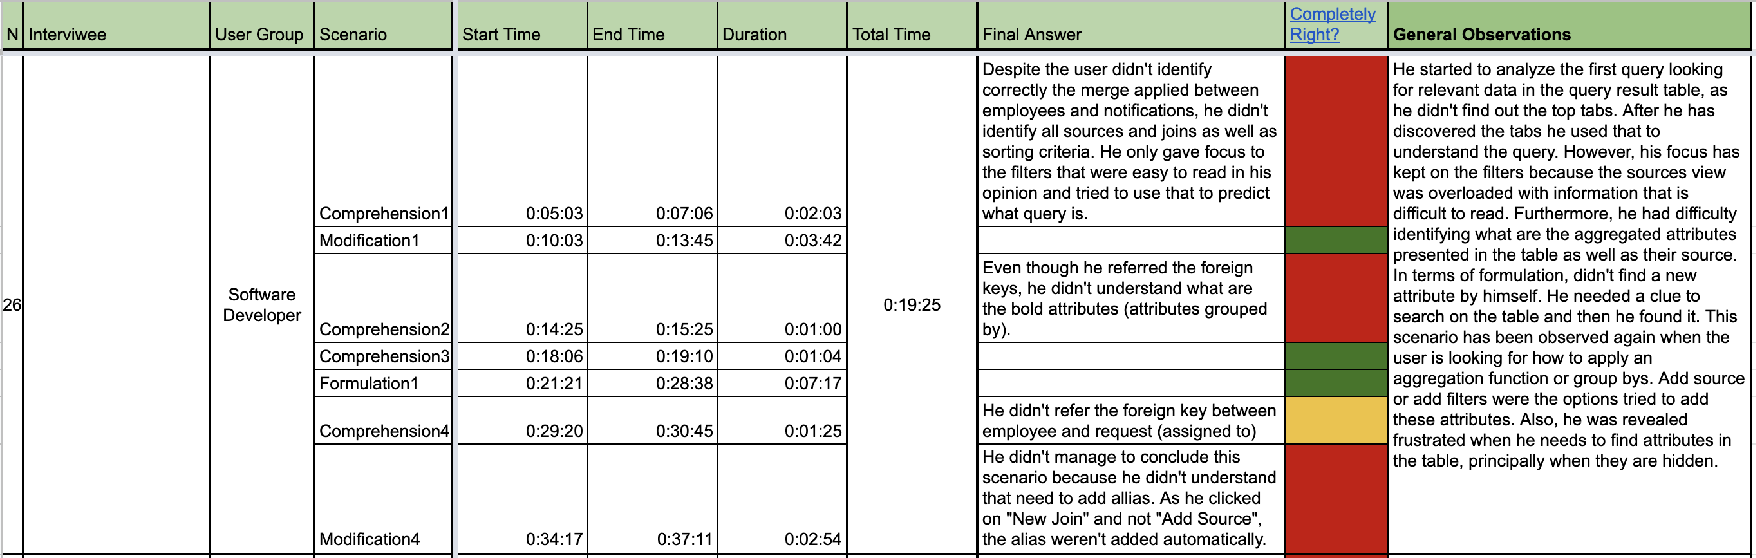
\includegraphics[height=1.9in]{user-evaluation-example}
	\caption{Example a general annotation registered after a usability test.}
	\label{fig:userEvaluationExample}
\end{figure}

\begin{table}[tb]
    \caption{Description of the effectiveness states considered.}
    \label{tab:effectiveness_states}
    \begin{tabular}{|l|l|l|l|}
        \hline
        \rowcolor[HTML]{C0C0C0} 
        \textbf{Legend}                                                                                                 & \textbf{Comprehension}                                                                                                                                                                                                                                                                                                             & \textbf{Modification}                                                  & \textbf{Formulation}                                                                   \\ \hline
        \cellcolor[HTML]{38761D}{\color[HTML]{FFFFFF} \textbf{Achieved}}                                                & \begin{tabular}[c]{@{}l@{}}When the user mentioned \\ all components of the queries \\ (sources, joins with foreign \\ keys, filters, sorting, aggregation \\ functions). The only thing that \\ would not be considered is if \\ the user didn't refer with or \\ without joins when they were \\ put automatically.\end{tabular} & All modifications                                                      & \begin{tabular}[c]{@{}l@{}}Completely \\ Right\end{tabular}                            \\ \hline
        \cellcolor[HTML]{F1C232}\textbf{\begin{tabular}[c]{@{}l@{}}Partially \\ Achieved\end{tabular}}                  & \begin{tabular}[c]{@{}l@{}}If the user didn't refer to the \\ foreign key between two tables \\ where there is more than one \\ foreign key between two tables. \\ The another possibility is if the \\ user did not specify only the \\ sorting criteria.\end{tabular}                                                            & \begin{tabular}[c]{@{}l@{}}Forgot to remove\\ some filter\end{tabular} & \begin{tabular}[c]{@{}l@{}}Group data \\ using the \\ wrong \\ identifier\end{tabular} \\ \hline
        \cellcolor[HTML]{CC0000}{\color[HTML]{FFFFFF} \textbf{\begin{tabular}[c]{@{}l@{}}Not \\ Achieved\end{tabular}}} & Anything else                                                                                                                                                                                                                                                                                                                      & Anything else                                                          & Anything else                                                                          \\ \hline
        \end{tabular}
    \end{table}


In addition, a text highlighting the most relevant usability test topics, including users' opinions, reactions, expectations, and suggestions has been included for each user. It was registered the qualitative result of the usability tests, which are not only important for the design of the next iterations but also to assess users' satisfaction.


Furthermore, other important details of each scenario were reported. In the comprehension scenarios, it was assessed the correct components of the query identified and the means used to perceive the solution. Regarding the formulation scenarios, the options used to build the query were identified and also the difficulties and the exploration of not supported options.

Finally, to gain a more extensive notion and some quantitative metrics about the interaction with the interfaces, the users were asked to fill in a System Usability Scale (SUS) \cite{system_usability_scale} as their final task in the usability test.

The process detailed in this chapter was used in all interfaces tested and addressed in this dissertation: the existing interface of Aggregates, the paper prototype, and the final prototype which was integrated into Service Studio (the Visual \gls{IDE} of the OutSystems Platform). The next chapter will describe the design and implementation process of each prototype built, but also how they were tested using the methodology referred.